% Условная компиляция для самостоятельной работы
\ifdefined\mainfile
    % Если это часть основного файла, не добавляем начало и конец документа
\else
    \documentclass[12pt, a4paper]{report}
    \usepackage{/Users/vladbelousov/Desktop/Semestr_4-FP-NSU/Настройка/library}
    \usepackage[utf8]{inputenc} % Подключение поддержки UTF-8
    \begin{document}
\fi

%%-------------------------------%%

Положение главных максимумов: 

\[ \sin ^2 \left( \frac{kD}{2 }  \sin \theta_m  \right) = 0 \Rightarrow \frac{kD}{2 }  \sin \theta_m = m \pi \Rightarrow \sin \theta_m = \theta_m = m \frac{\lambda}{D}  \] 

\begin{center}
    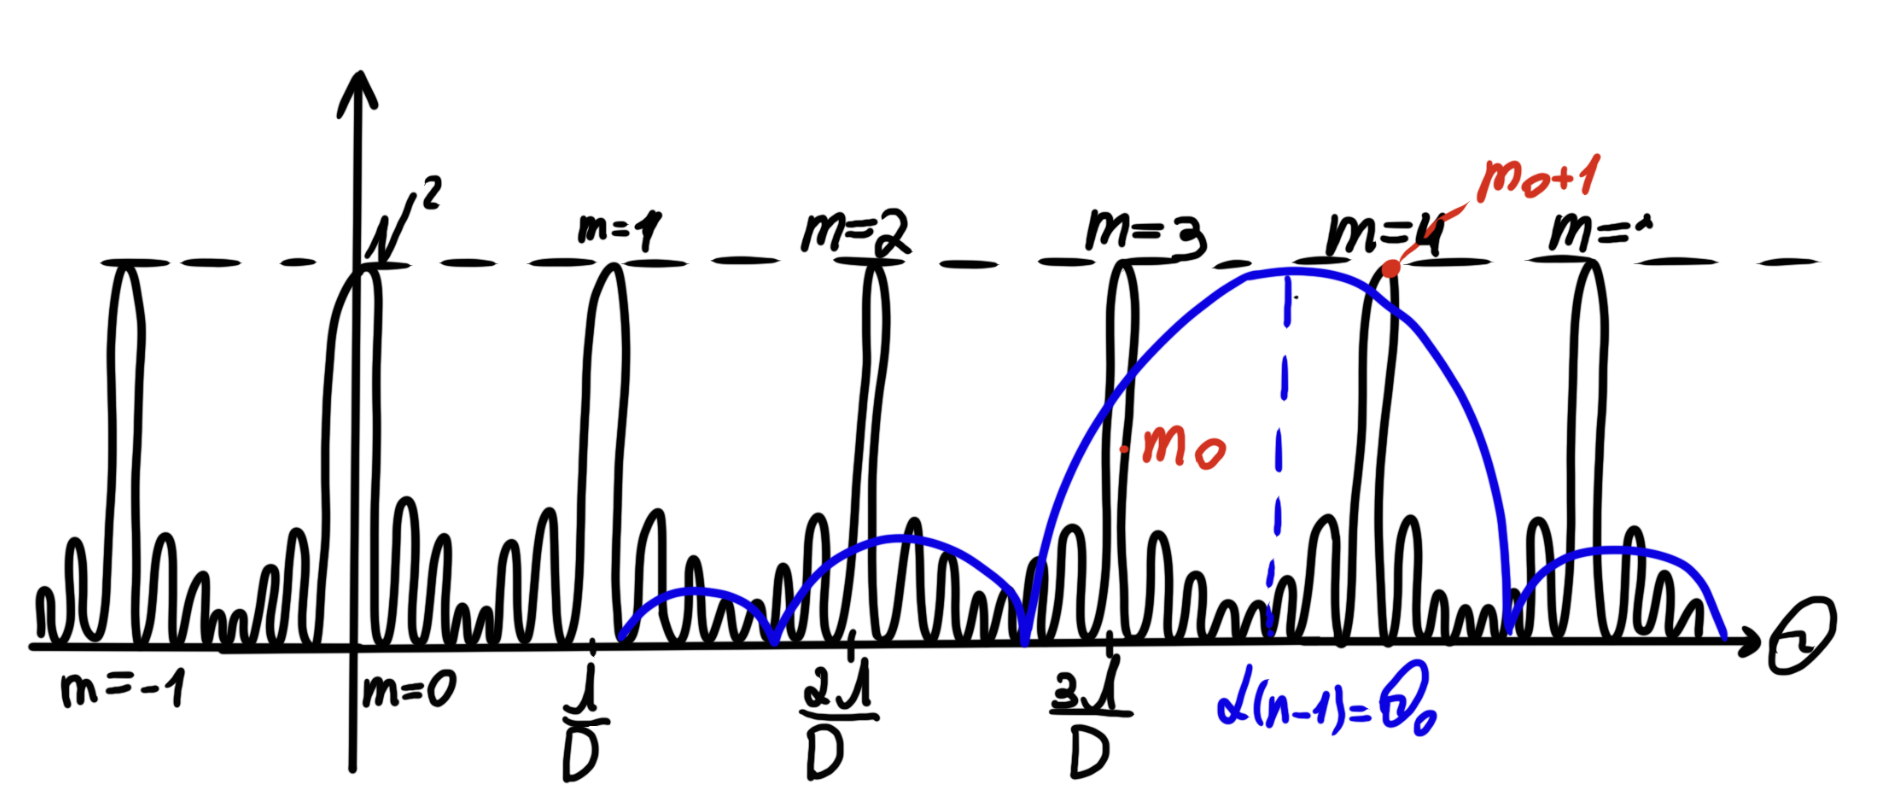
\includegraphics[width=0.7\textwidth]{/Users/vladbelousov/Desktop/Semestr_4-FP-NSU/ЭиО/Лекции_по_дням/image/144.png}
\end{center}

\[ \sin \theta_0 = \alpha (n-1 ) \ll 1 \Rightarrow \theta_0 = \alpha (n-1 ) \] 

Обращение в ноль: \(  \displaystyle  \frac{kD}{2 }  (\alpha (n-1 ) - (\theta_0 - \Delta \theta )) = \pm \pi \Rightarrow \Delta \theta = \pm \frac{\lambda}{D}  \) 

\[ m_0 = \left[ \frac{\alpha (n -1 )}{ \frac{\lambda}{D} }  \right] \] 

\( \delta \theta_{ int }   \) - ширина главного максимума = \( \displaystyle  \frac{\Delta \theta_m }{\frac{\lambda}{D } } = \frac{\lambda}{DN}   \) 


\section{Основные параметры диффракционных решеток}

1. Угловая дисперсия: \( \displaystyle \frac{ d \theta_m }{d \lambda }  = \frac{d }{d \lambda } \left( m \frac{\lambda}{D}  \right) = \frac{m}{D }  = \frac{\theta_m }{\lambda }   \)   - для фазовой решетки \( \frac{d \theta }{ d \lambda }\sim  \frac{ \theta_{m_ 0} }{\lambda}   \) 

2. Свободная область дисперсии  \( \Delta \lambda  \) 

(для фазовой решетки)

\begin{center}
    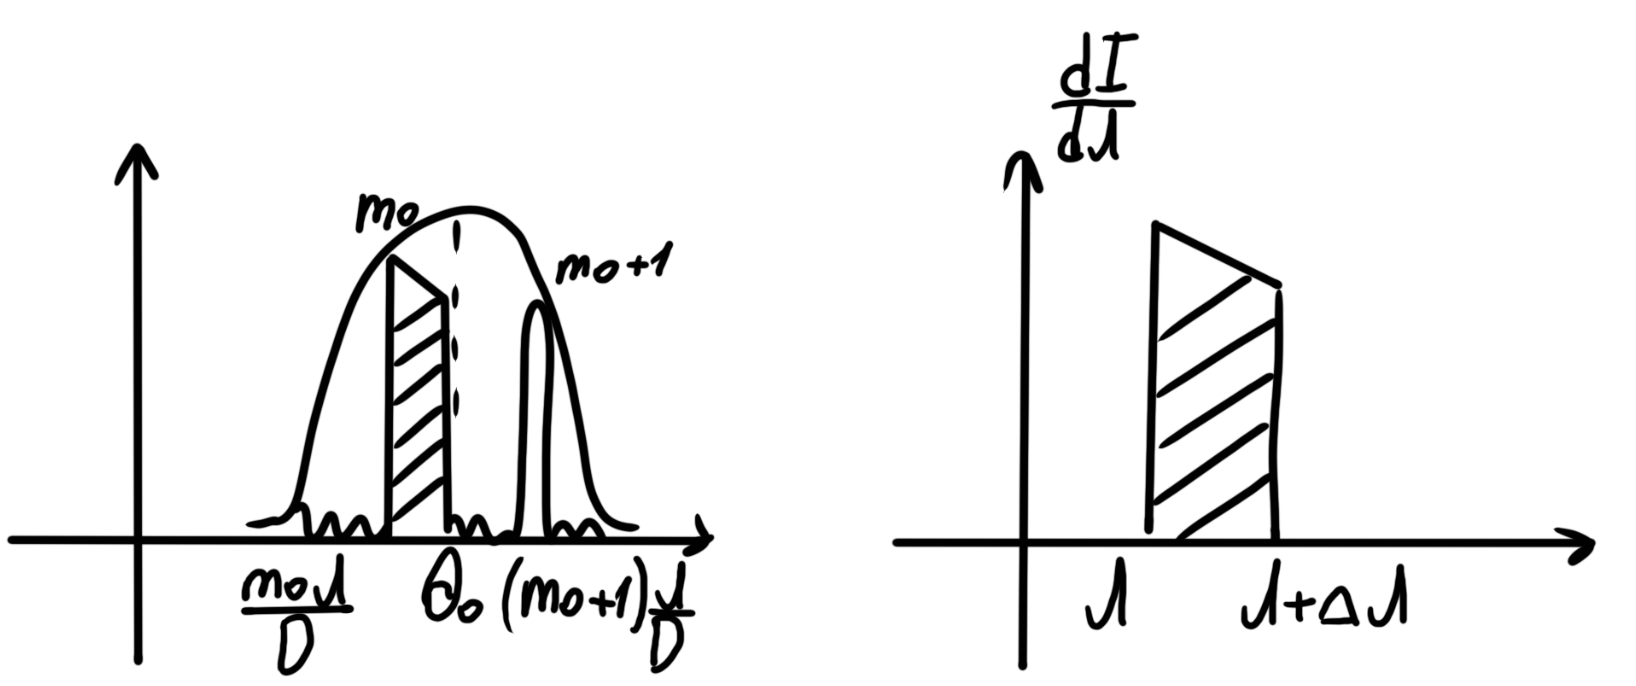
\includegraphics[width=0.7\textwidth]{/Users/vladbelousov/Desktop/Semestr_4-FP-NSU/ЭиО/Лекции_по_дням/image/145.png}
\end{center}

\[ \lambda ' = \lambda \pm  \lambda+ \Delta \lambda \] 

\begin{center}
    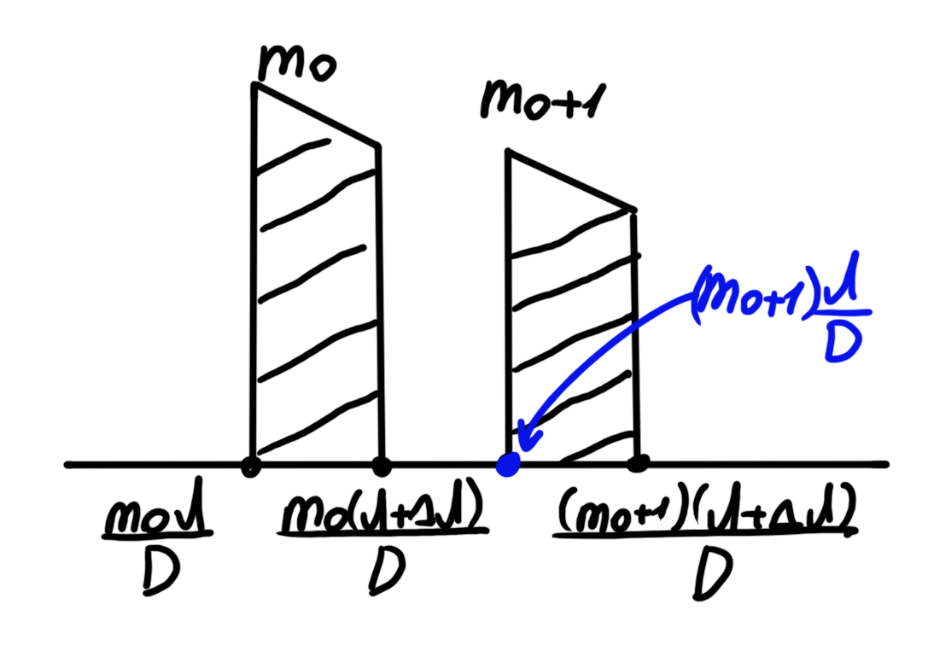
\includegraphics[width=0.5\textwidth]{/Users/vladbelousov/Desktop/Semestr_4-FP-NSU/ЭиО/Лекции_по_дням/image/146.png}
\end{center}

\[ \Delta \lambda _{\max  } - ? \quad  \frac{ m_0 (\lambda + \Delta \lambda )}{D }  \le  (m_0 +1 ) \frac{\lambda}{D }  \Rightarrow m_0 \Delta \lambda  \le  \lambda    \] 
\[ \Rightarrow \Delta \lambda _{ \max  } = \frac{\lambda}{m_0 } \text{ - свободная область дисперсии}  \] 

3. Спектральное разрешение \( \displaystyle  R_{\lambda } = \frac{\lambda}{\delta \lambda_{ \min  } }   \) 

(для фазовой решетки)

\[ \frac{m_0 \lambda_1 }{D } +\underbrace{ \delta \theta_{ int }}_{\frac{\lambda_1 }{D N} } = \frac{ m_0 \lambda_2 }{D } = \frac{m_0 (\lambda_1 + \delta \lambda_{ \min  } )}{ D}     \] 
\[ \frac{\lambda_1}{D N }  = \frac{m_0 \delta \lambda_{ \min  } }{D }  \] 

\[ R_{\lambda } = \frac{\lambda}{\delta \lambda_{ \min  } } = m_0 N   \] 
, где \( N \) - типичное \( 10^5 \), \( m_0 = 1 \pm 100 \) 

\section{Принцип Гюйгенса-Френеля и геометрическая оптика}

На линзу падает плоская монохроматическая волна под малым углом к \( Oz \) 

\begin{center}
    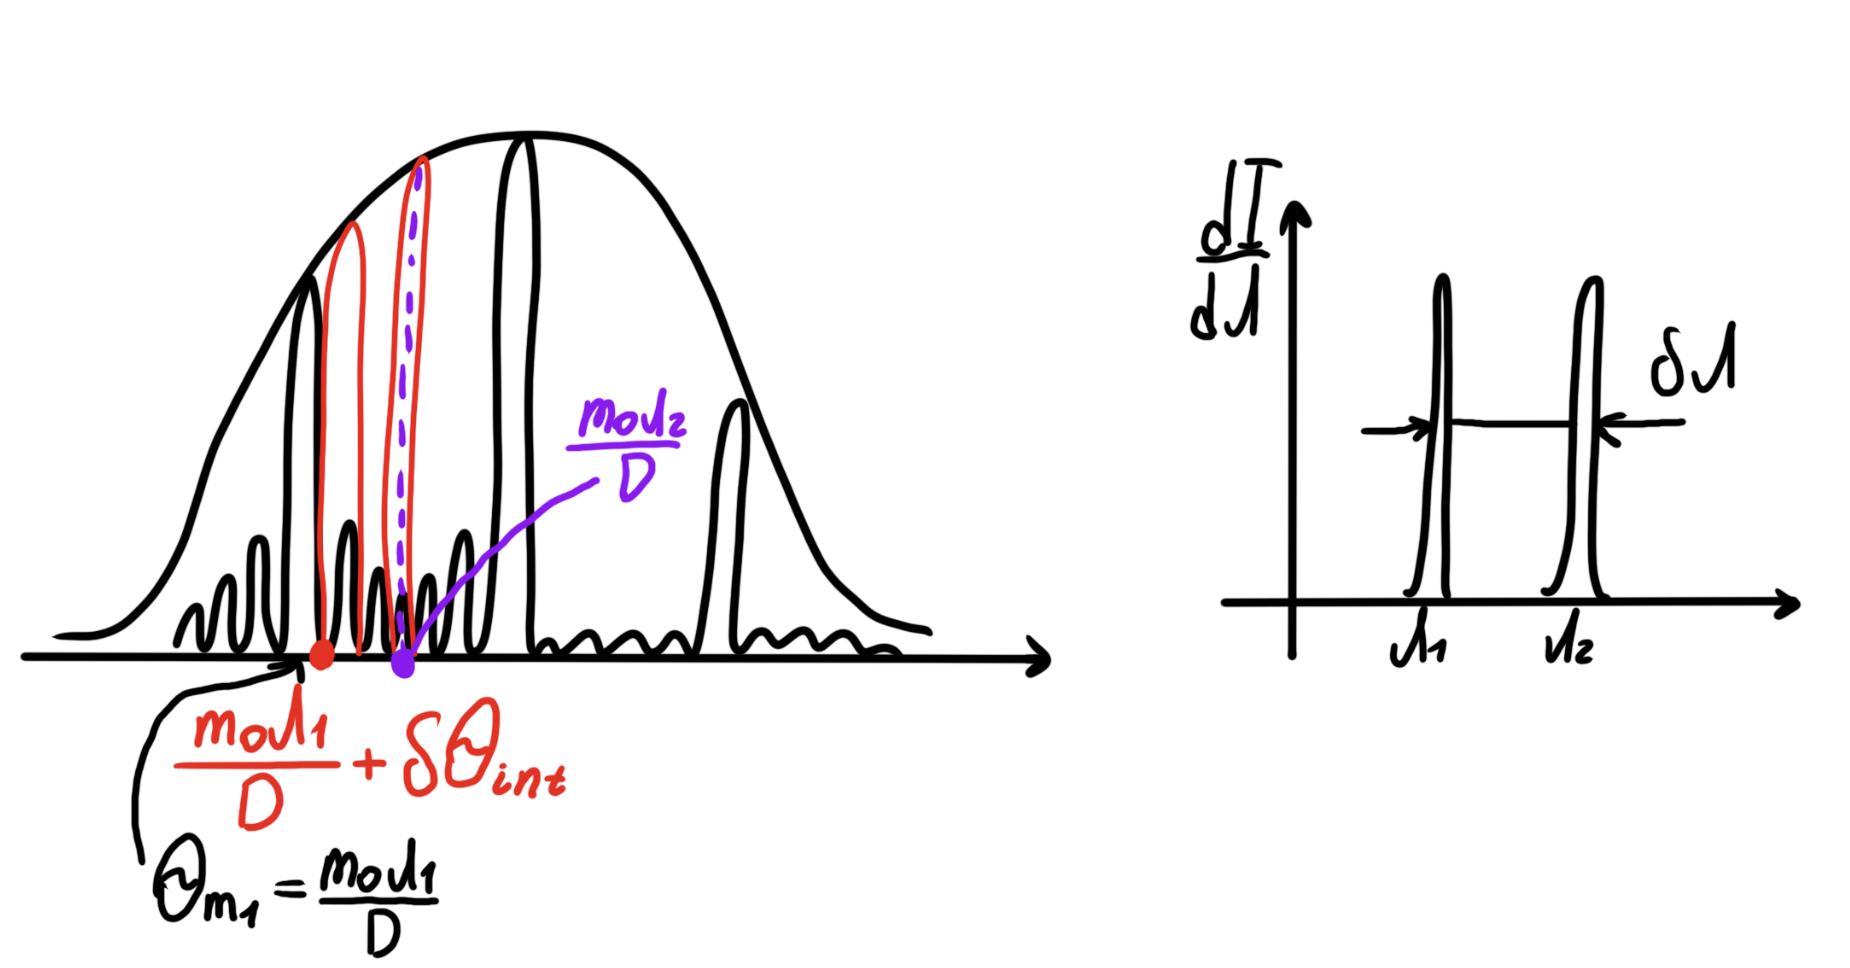
\includegraphics[width=0.7\textwidth]{/Users/vladbelousov/Desktop/Semestr_4-FP-NSU/ЭиО/Лекции_по_дням/image/147.png}
\end{center}
\( R_1 >0 ,\text{ }  R_2 <0 \) 

\[ \varphi (r ) _{\text{на оп}_2 } = k S_{\text{оптический путь} }   = k (\Delta_1 + \Delta_2 + (d_0 - \Delta_1 - \Delta_2 )n ) =\underbrace{ k d_0 n}_{\varphi_0} - k (n-1 ) (\Delta_1 + \Delta_2 ) \] 

\begin{center}
    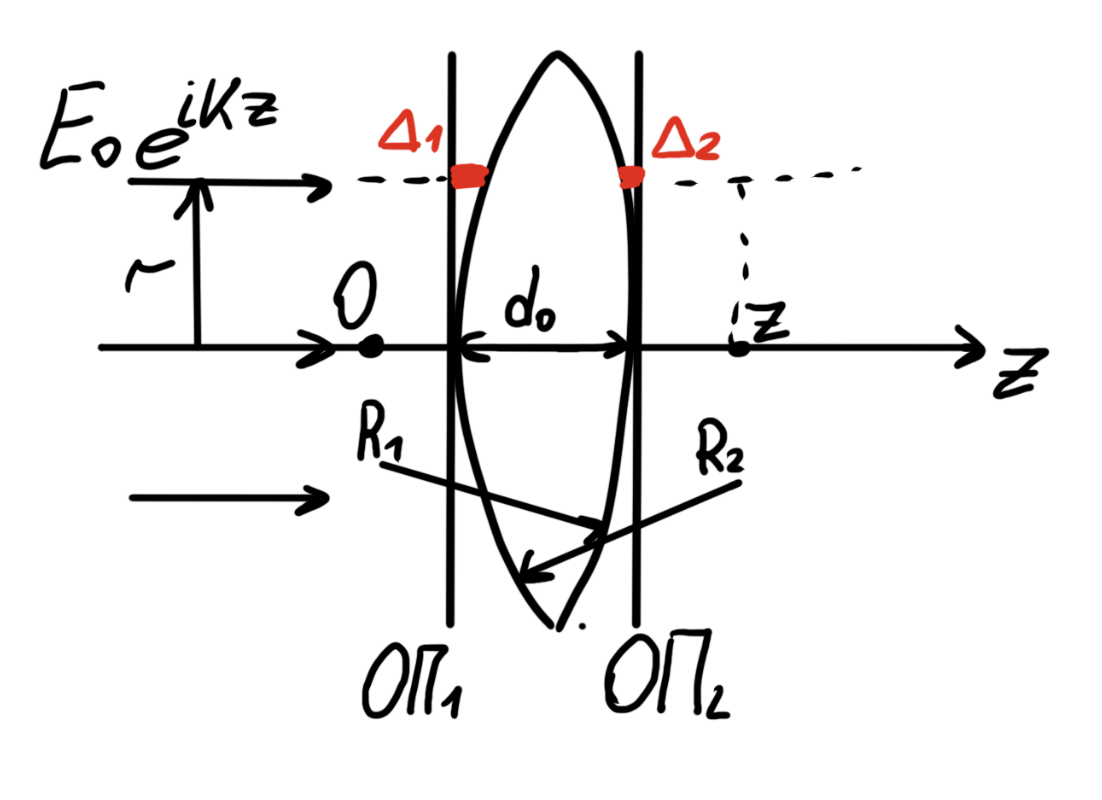
\includegraphics[width=0.5\textwidth]{/Users/vladbelousov/Desktop/Semestr_4-FP-NSU/ЭиО/Лекции_по_дням/image/148.png}
\end{center}

\[ \Delta z = \sqrt{R_1 ^2 - r ^2 } \Rightarrow \Delta_1 = R_1 - \Delta z = R_1 - \sqrt{R_1 ^2 - r ^2 }  \] 

Если углы малы \(\Rightarrow r \ll R_1 ,R_2   \) 
\[ \Rightarrow \Delta_1 = R_1 - R_1 \left( 1 - \frac{r ^2 }{2 R_1 ^2 }  \right) = \frac{ r ^2 }{2 R_1 }  \] 
\[ \Delta_2 = \frac{ r ^2 }{2 (- R_2 )} \Rightarrow \varphi(r ) = \varphi_0 - k \frac{ r ^2 }{2 } (n-1 ) \left( \frac{1}{R_1 } - \frac{1}{R_2}   \right)  = \varphi_0 - \frac{k r ^2 }{2 F_{\text{л} } }    \] 
, где \( F_{\text{л} }  \) - фокусное расстояние линзы. 

\[ \varphi (r, z ) = \varphi_0 - \frac{k r ^2 }{2 F_{\text{л} } } + (z - d_0 ) k \text{ на поверхности фазового фронта } \varphi (r, z ) = \mathrm{ const}    \] 

\begin{center}
    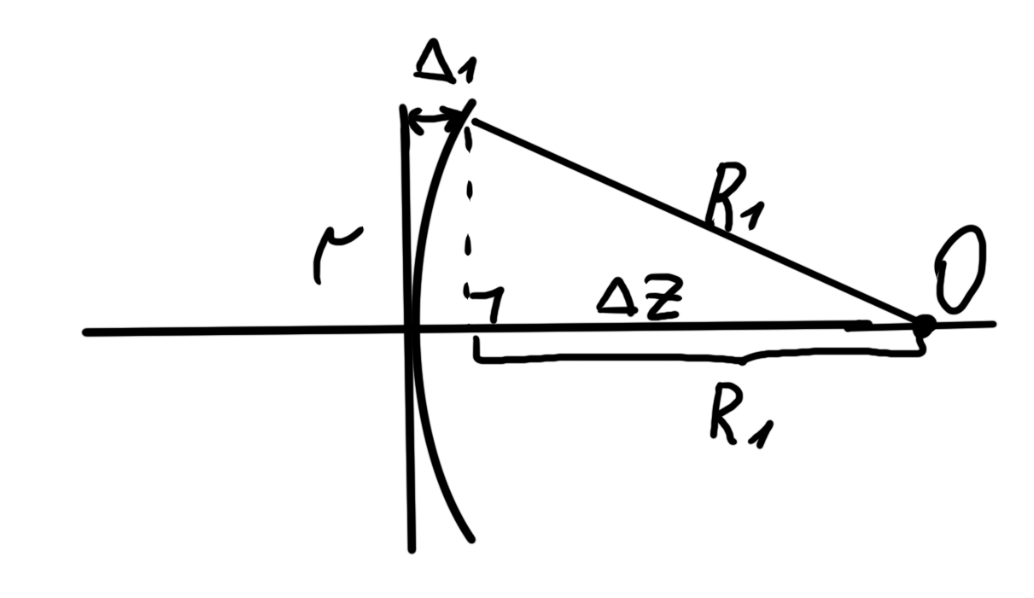
\includegraphics[width=0.5\textwidth]{/Users/vladbelousov/Desktop/Semestr_4-FP-NSU/ЭиО/Лекции_по_дням/image/149.png}
\end{center}
Параболоид вращения \( z = \mathrm{const }  + \displaystyle  \frac{ r ^2 }{2 F_{\text{л} } }   \) 

Параболоид и сфера близки в параксиальном приближении. 

\[ \text{В точке: }  \frac{d z }{d r } = 0 \quad  \frac{1}{R_{\text{кр} } } = \frac{ d ^2  z }{ d r ^2  } = \frac{d ^2 }{dr ^2 }   \left( \frac{ r ^2 }{2 F_{\text{л} } }  \right)   = \frac{1}{F_{\text{л} } }  \Rightarrow R_{\text{кр} } = F _{\text{л }  }  \] 

\begin{center}
    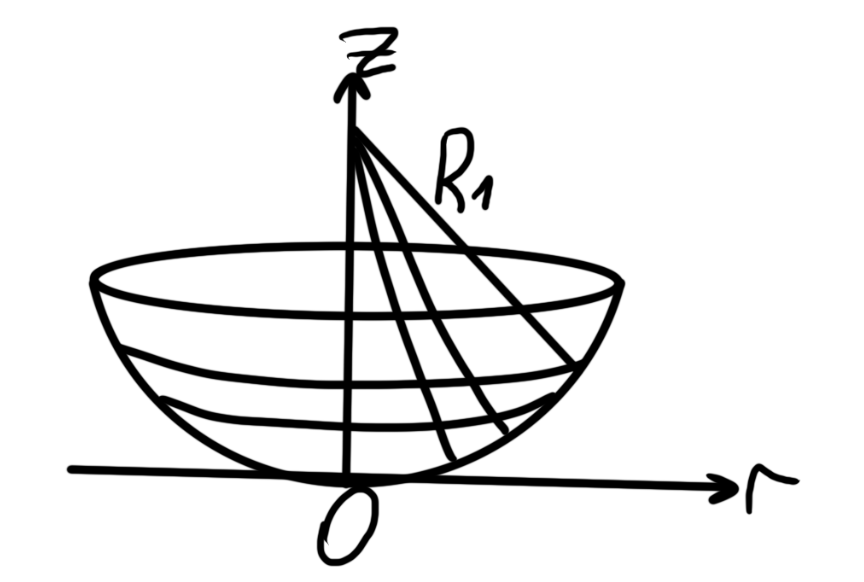
\includegraphics[width=0.45\textwidth]{/Users/vladbelousov/Desktop/Semestr_4-FP-NSU/ЭиО/Лекции_по_дням/image/150.png}
\end{center}

Изображение  точечного источника линзой с учетом дифракции на линзе. 

\[ r_1 = \sqrt{(x_l - x_s ) ^2 + (y_l - y _s ) ^2 + a ^2 } , \quad \] 
\[ r_2 = \sqrt{x_p - x_l  ^2 + (y_p - y_l ) ^2 + b ^2  } \] 

\[ \left\lvert a  \right\rvert \left\lvert b  \right\rvert \gg \left\lvert x_l     \right\rvert, \left\lvert x_s  \right\rvert , \left\lvert y_l  \right\rvert , \left\lvert y_s  \right\rvert, \left\lvert y_p  \right\rvert, \left\lvert x_p \right\rvert   \text{ - параксиальное приближение}  \] 

\begin{center}
    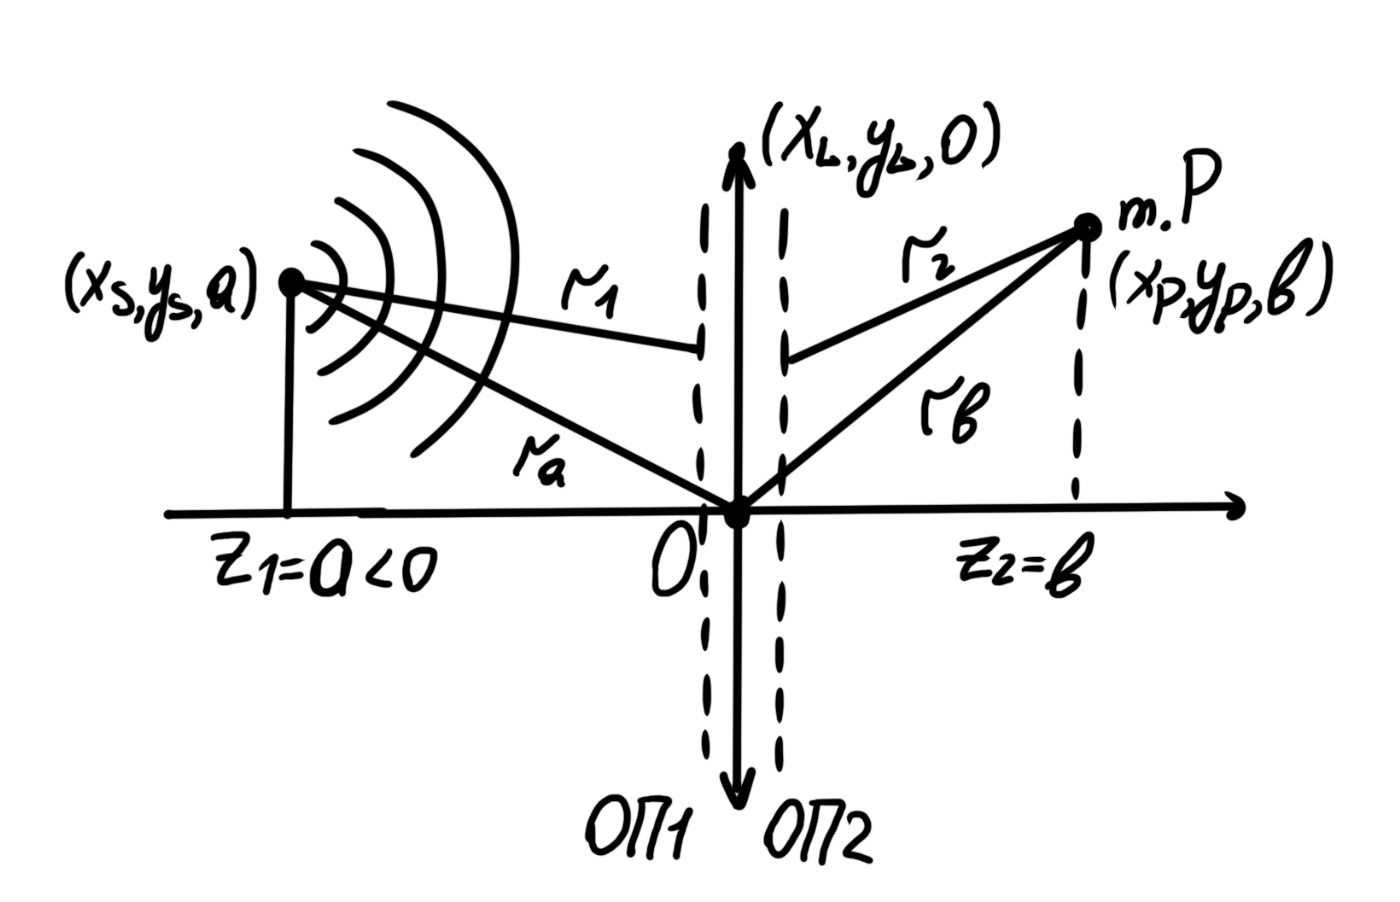
\includegraphics[width=0.7\textwidth]{/Users/vladbelousov/Desktop/Semestr_4-FP-NSU/ЭиО/Лекции_по_дням/image/151.png}
\end{center}

\[ \text{На ОП}_1 : E_1 (x_2,y_2, 0) = \frac{A}{r_1 } e^{i k r_1 }    \] 
\[ r_1 \approx \left\lvert a  \right\rvert \left(  1 + \frac{ (x_l - x_s) ^2 }{2 a^2} + \frac{(y_l - y_s ) ^2 }{2 a ^2 } +...    \right) = \left\lvert a  \right\rvert - \frac{(x_l - x_s ) ^2  + (y_l + y_s) ^2 }{2a }  \] 
\[ E_1(x_l, y_l , 0 ) = E_0 e^{ i k \left\lvert a  \right\rvert} e^{ - i k \frac{ (x_l - x_s ) ^2 + (y_l - y_s) ^2   }{2a } }    \] 

\[ \text{На ОП}_2: E_2 (x_l , y_l , 0 ) = E_1 (x_l, y_l , 0 ) e^{i \varphi_0 - ik \frac{x_l ^2 + y_l ^2 }{2 F_{\text{л} } } }   \] 

В плоскости \( z =b : \) 

\[ E_p (x_p , y_p , 0 ) = \frac{k}{ 2 \pi i } \int_{- \frac{D}{2 } }^{\frac{D}{2 }  }\int_{-\frac{D}{2 } }^{\frac{D}{2 } } d x_l dy _l E_2(x_l , y_l ,0 ) \frac{e^{i k r_1 } }{r_2 } \cos \theta      \] 

\[ r_2 = b + \frac{ (x_p - x_l ) ^2 + (y_p - y_l ) ^2 }{2 b }  \] 

\[ E_p = \frac{k E_0 }{2 \pi  i b } e^{ik \left[ -a - \frac{ x_s ^2 + y_s ^2 }{2a } +b + \frac{ x_p ^2 + y_p ^2 }{2b }   \right] +i \varphi_0}  \int_{-\frac{D}{2 } }^{\frac{D}{2 }  }   dx_l e^{ik \left[ - \frac{x _l ^2 }{2a } - \frac{x_l ^2 }{2 F_{\text{л} } } + \frac{x_l ^2}{2 b }   + \frac{ x_s \cdot x_l }{a } - \frac{ x_p \cdot x_l }{b}      \right]} \cdot \int_{-\frac{D}{2 } }^{\frac{D}{2 }  d y_l (... )}  \] 
, где \( \displaystyle r_a = -a \frac{ x_s ^2 +y _s ^2}{2a } ,\text{ }  r_b = b + \frac{ x_p ^2 + y_p ^2 }{2 b}   \) 

Если \( b \)-координата плоскости изображения, то \( \displaystyle  \frac{1}{a }  + \frac{1}{F_{\text{л} } } = \frac{1}{b}   \) 

\[ E_p = \frac{E_0}{i \lambda b } e^{ik (r_a +r_b ) + i \varphi_0 } D \cdot \frac{ e^{ik \left( \frac{x_s }{a} - \frac{x_p}{b}  \right)\frac{D}{2 } } - e^{- ik \left( \frac{x_s }{a }  - \frac{x_p}{b}   \right)\frac{D}{2 } }  }{2i k \left( \frac{x_s}{a } - \frac{x_p}{b}   \right)\frac{D}{2} } \cdot (\text{по }y )    \] 

\[ I_p = \frac{\left\lvert E_p  \right\rvert ^2 }{2 } = I_0 \underbrace{\frac{ D ^4 }{\lambda ^2 b ^2 }}_{P_{\text{Ф} } ^2 } \mathrm{sinc } ^2 \left( \frac{kD}{2 }  \left( \frac{x_s  }{a } - \frac{x_p}{b}   \right) \right) \mathrm{sinc  } ^2 \left( \frac{kD}{2 } \left( \frac{y_s }{a } - \frac{y_p}{b}   \right) \right)      \] 
\[ \frac{x_s}{a }  - \frac{x_{ p_0 } }{b } =0 \Rightarrow \begin{aligned}
    x_{ p_0 } = x_s \frac{b}{a }  <0  \\
    y_{ p_0 } = y_s \frac{b}{a }  <0 
\end{aligned}   \] 

\begin{center}
    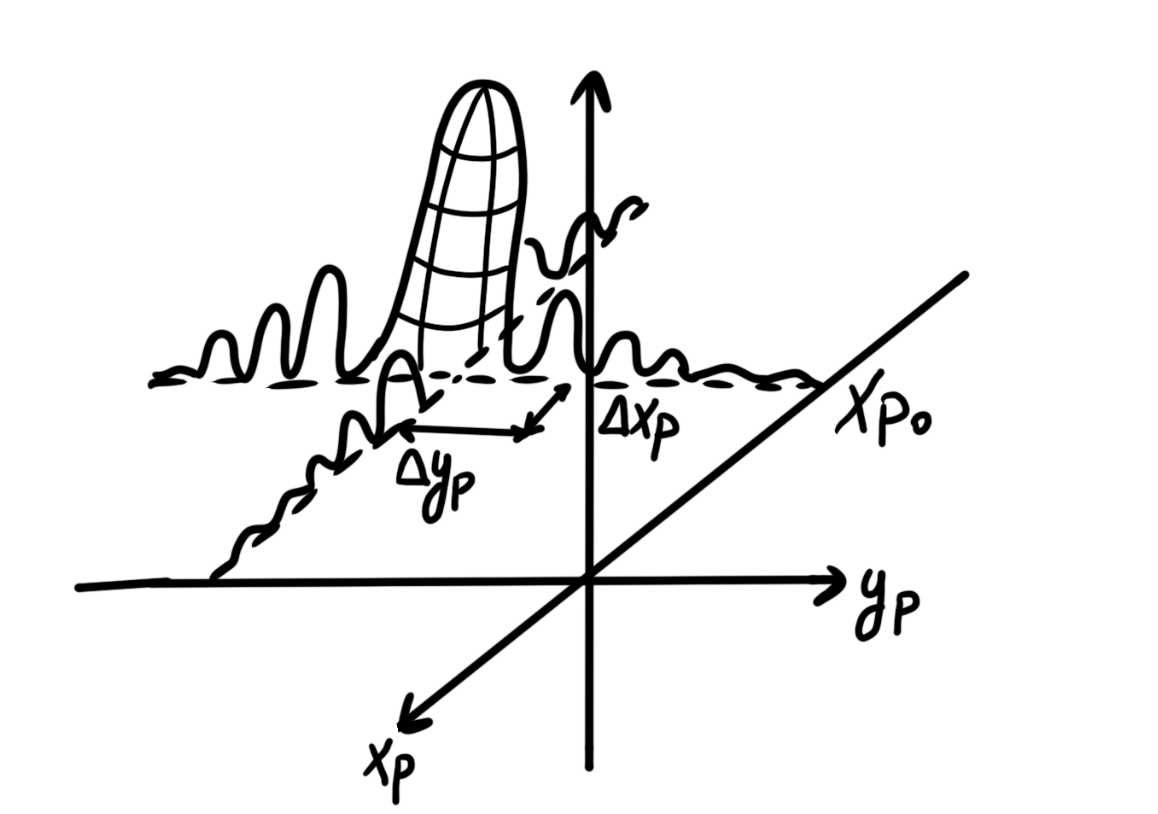
\includegraphics[width=0.7\textwidth]{/Users/vladbelousov/Desktop/Semestr_4-FP-NSU/ЭиО/Лекции_по_дням/image/152.png}
\end{center}

Размер пятна по \( x \): \( \displaystyle  \frac{kD}{2 } \left( \frac{x_s}{a }  - \frac{x_{ p_0 } +\Delta x_p        }{b}  \right) = \pm  \pi \)  

\[ \begin{aligned}
\Delta x_p = \frac{\lambda}{D } b \\ 
\Delta y_p = \frac{\lambda}{D } b
\end{aligned} \] 

\[ I_{ \max  } = I_0 P_{\text{Ф} } ^2; \text{ для фотоаппарата }  D \sim 1 , \text{ }  \lambda \sim  0,5 \cdot 10 ^{-4 } , \text{ }  b \sim  5 \text{ см }    \] 

\[ P_{\text{Ф} } = \frac{1 ^2 }{0, 5 \cdot 10^{-4} \cdot 5 }  = 4 \cdot 10^3  \Rightarrow P_{\text{Ф} } ^2 = 1,6 \cdot 10^{7}     \] 
\[ a_m \sqrt{m \lambda b } = 0,5 \text{ см}= \sqrt{m  \cdot 5 \cdot 10^{-4} \cdot 5       } \Rightarrow m = 1000  \] 

%%-------------------------------%%

% Закрытие документа, если файл компилируется отдельно
\ifdefined\mainfile
    % Если это основной файл, не нужно заканчивать документ
\else
    \end{document}
\fi